\documentclass[10pt]{beamer}



\usetheme[progressbar=frametitle]{metropolis}
\usepackage{appendixnumberbeamer}
\usepackage{lipsum}
\usepackage{amsmath}
\usepackage{amssymb}
\usepackage{booktabs}
\usepackage{url}
\usepackage[utf8]{inputenc}
\usepackage[english]{babel}
\usepackage[scale=2]{ccicons}
\usepackage{pgfplots}
\usepgfplotslibrary{dateplot}
\usepackage{dirtytalk}
\usepackage{xspace}
\usepackage{listings}
\usepackage{xcolor}
\usepackage{tikz}
\usepackage{animate}
\usepackage{picture}
\definecolor{codegreen}{rgb}{0,0.6,0}
\definecolor{codegray}{rgb}{0.5,0.5,0.5}
\definecolor{dodger}{RGB}{30, 144, 255}
\definecolor{floral}{RGB}{242, 243, 244}
\lstdefinestyle{mystyle}{
    backgroundcolor=\color{floral},
    commentstyle=\color{codegreen},
    morekeywords={as},
    keywordstyle=\color{orchid},
    numberstyle=\tiny\color{codegray},
    stringstyle=\color{dodger},
    basicstyle=\ttfamily\footnotesize,
    breakatwhitespace=false,
    breaklines=true,
    captionpos=b,
    keepspaces=true,
    numbers=left,
    numbersep=5pt,
    showspaces=false,
    showstringspaces=false,
    showtabs=false,
    tabsize=2
}
\lstset{style=mystyle}
\newcommand{\themename}{\textbf{\textsc{metropolis}}\xspace}
\definecolor{mpigreen}{HTML}{007977}
\definecolor{orchid}{RGB}{186, 85, 211}
\setbeamercolor{frametitle}{bg=white, fg=black!80}
\setbeamercolor{background canvas}{bg=white}
\DeclareMathOperator*{\argmax}{arg\,max}
\newcommand{\magenta}[1]{\textcolor{magenta}{#1}}

\usepackage{ulem}
\usepackage[subpreambles=true]{standalone}
\title{Langage Python}
\subtitle{ISUP, Sorbonne Université}
\author{Etienne Guével Ingénieur de Recherche - SCAI \footnotesize{etienne.guevel@sorbonne-universite.fr}}
\date{Septembre-Novembre 2025}
\titlegraphic{\hfill
\includegraphics[height=1.5cm]{img/logo_sorbonne.png}}


\begin{document}
 
\maketitle

\begin{frame}{}
  \centering
  \Large
  \textbf{Partie 2}

  \textbf{Programmation objet}
\end{frame}

\section{Concepts de la programmation objet}




\begin{frame}{Introduction}

  \begin{block}{En python}
    \medskip
    \begin{itemize}
      \item<+-> Les données sont représentées sous forme d'objets ou par des relations entre les objets
      \item<+-> Chaque objet possède un \textcolor{red}{identifiant}, un \textcolor{blue}{type} et une \textcolor{orange}{valeur}
      \item<+-> La fonction \texttt{id} revoie l'entier représentant cet identifiant
      \item<+-> L'identifiant d'un objet ne change jamais après sa création et représente l'adresse mémoire où est stockée l'objet
      \item<+-> L'opérateur \texttt{is} compare les identifiants de deux objets
      \item<+-> Les objets créés par l'utilisateur sont \textbf{mutables} par défaut
    \end{itemize}
  \end{block}

\end{frame}



\begin{frame}{Introduction}

  \begin{block}{Définition}
    \medskip
    En informatique, un objet est un conteneur symbolique qui contient des informations et des mécanismes concernant un sujet

    C'est une sorte d'abstraction du monde réel définie par un \textbf{ensemble de caractéristiques} (\underline{attributs} et \underline{méthodes}).
  \end{block}

  \textcolor{blue}{Par exemple, un oiseau est un canard s'il vole comme un canard, s'il cancane comme un canard et s'il nage comme un canard.}
\end{frame}


\begin{frame}{Programmation objet vs procédurale}

  \begin{minipage}[t]{0.48\textwidth}
  \textbf{Programmation procédurale}
  \begin{itemize}
    \item<1-> Basée sur des procédures (séquences d'instructions, appels de fonctions)
    \item<2-> Exécutions étape par étape
    \item<3-> Les données et méthodes sont susceptibles de changer durant l'exécution
  \end{itemize}
  \end{minipage}
  \hfill
  \begin{minipage}[t]{0.48\textwidth}
  \textbf{Programmation objet}
  \begin{itemize}
    \item<1-> Basée sur des classes
    \item<3-> Les données sont fixées dans la définition même des classes
    \item<4> C'est une manière de stocker de l'information
  \end{itemize}
  \end{minipage}
\end{frame}


\begin{frame}{Concepts de la programmation objet}
  \begin{block}{Concepts abordés dans cette partie}
    \medskip
    \begin{itemize}
      \item<+-> Classe 
      \item<+-> Constructeur, attributs et méthodes 
      \item<+-> Principe d'encapsulation
      \item<+-> Héritage
    \end{itemize}
  \end{block}
\end{frame}






\begin{frame}[fragile]{Classe vs objet}
  \begin{block}{Définition}
    \medskip
    Une classe est un bloc de code définissant l'ensemble des caractéristiques communes à plusieurs objets.\\
    C'est une sorte de plan permettant de créer plusieurs objets.
  \end{block}
\bigskip
\begin{lstlisting}[language=Python, numbers=none]
class Point():
    def __init__(self, x, y):
        self.x = x
        self.y = y
\end{lstlisting}

\end{frame}


\begin{frame}[fragile]{Contructeur}

  \begin{block}{Définition}
    \medskip

    Le constructeur est une fonction appelée lors de la création de l'objet.
    Elle permet d'allouer la mémoire nécessaire à l'objet et d'initialiser ses attributs.

    \medskip
    Le constructeur est une fonction définie par le mot clé \texttt{\_\_init\_\_}
  \end{block}
\begin{lstlisting}[language=Python, numbers=none]
def __init__(self, x, y):
    self.x = x
    self.y = y
\end{lstlisting}
\end{frame}



\begin{frame}[fragile]{Instanciation}

  \begin{block}{Définition}
    \medskip
    Une instance de classe est un objet dont le comportement et l'\textbf{état} sont définis dans la classe.

    L'instanciation est l'action de créer un objet à partir d'un modèle (c-à-d la classe) via deux opérations :
    \begin{itemize}
      \item l'\textcolor{red}{allocation} qui consiste à réserver un espace mémoire pour stocker l'objet
      \item l'\textcolor{red}{initialisation} qui consiste à fixer l'\textbf{état} de l'objet par l'appel au constructeur de la classe
    \end{itemize}

  \end{block}
\begin{lstlisting}[language=Python, numbers=none]
point = Point(x=1, y=2)
\end{lstlisting}
\end{frame}


\begin{frame}[fragile]{Attributs d'instance}

  \begin{block}{Définition}
    \medskip
    Les attributs sont des entités qui définissent les propriétés d'un objet. Dans l'exemple, \texttt{x} et \texttt{y} sont les attributs. Ils sont stockés dans la classe via le mot clé \texttt{self}
  \end{block}

\begin{lstlisting}[language=Python, numbers=none]
class Point():
    def __init__(self, x, y):
        self.x = x
        self.y = y
\end{lstlisting}

\onslide<2>
\begin{center}
  \boxed{\mbox{On parle d'attribut d'instance}}
\end{center}

Attributs de classe : voir \href{https://docs.python.org/3/tutorial/classes.html#class-and-instance-variables}{ici}

\end{frame}


% \begin{frame}[fragile]{Attributs de classe}

%   \begin{block}{Définition}
%     \medskip
%     Les attributs de classe sont des entités indépendantes de l'objet créé et dont la valeur est commune à tous les objets
%   \end{block}

% \begin{lstlisting}[language=Python, numbers=none]
% class Point():
%     point_type = "2D"
%     def __init__(self, x, y):
%         self.x = x
%         self.y = y
% \end{lstlisting}
% \end{frame}





\begin{frame}[fragile]{Méthodes d'instance}

  \begin{block}{Définition}
    \medskip
    Les sont des fonctions membres d'une classe. Elles permettent d'\textbf{intéragir avec l'état} de l'objet, en particulier le modifier.

  \end{block}
\begin{lstlisting}[language=Python, numbers=none]
class Point():
    def __init__(self, x, y):
        self.x = x
        self.y = y

    def norm(self):
        return math.sqrt(self.x**2 + self.y**2)
\end{lstlisting}

Méthodes de classe : voir \href{https://www.geeksforgeeks.org/class-method-vs-static-method-python/}{ici}

\end{frame}


% \begin{frame}[fragile]{Méthodes de classe}

%   \begin{block}{Définition}
%     \medskip
%     Comme les attributs de classe, les méthodes de classe sont partagées entre plusieurs objets d'une même classe. Elles définissent les caractéristiques de la classe et n'agissent pas sur l'état des objets.

%     Les méthodes de classe ont accès aux attributs de classe et non aux attributs d'instance
%   \end{block}
% \begin{lstlisting}[language=Python, numbers=none, morekeywords={@classmethod}]
% class Point():
%     point_type = "2D"
%     def __init__(self, x, y):
%         ...

%     def norm(self):
%         return math.sqrt(self.x**2 + self.y**2)

%     @classmethod
%     def print_type(cls):
%         print(f"My type is {cls.point_type}")
% \end{lstlisting}
% \end{frame}





\begin{frame}[fragile]{Méthodes statiques}

  \begin{block}{Définition}
    \medskip
    Les méthodes statiques n'ont accès ni aux attributs de classe, ni aux attributs d'instance. Elles ont un lien logique avec la classe et l'objet mais ne nécessitent pas la connaissance des états.

    Par exemple, elles peuvent servir de fonctions utilitaires

  \end{block}
\begin{lstlisting}[language=Python, numbers=none, morekeywords={@staticmethod}]
class Point():
    def __init__(self, x, y):
        self.x = x
        self.y = y
        print(self.to_string(x, y))

    @staticmethod
    def to_string(x, y):
        return f"""
        x = {x}
        y = {y}         
        """
\end{lstlisting}
\end{frame}



\section{Principe d'encapsulation}

\begin{frame}[fragile]{Principe d'encapsulation}

  \onslide<1->
  Le principe d'encapsulation est un des concepts fondammentaux en programmation objet. Il s'agit de \textcolor{red}{regrouper des données} dans un objet pour en \textcolor{red}{limiter la manipulation}, qui se fait uniquement par des méthodes dédiées.

  Les méthodes sont ainsi vues comme une interface destinée à l'utilisateur, ou une sorte de couche de protection vis-à-vis de l'accès aux données

  \onslide<2->
  Le principe d'encapsulation est fortement lié à la \textcolor{red}{portée des méthodes} et des attributs (publique, protégée ou privée).
% \textcolor{red}{En programmation, l'encapsulation désigne le regroupement de données avec un ensemble de routines
% qui en permettent la lecture et la manipulation. Ce principe est souvent accompagné du masquage
% de ces données brutes1 afin de s'assurer que l'utilisateur ne contourne pas l'interface qui lui est destinée.
% L'ensemble se considère alors comme une boite noire ayant un comportement et des propriétés spécifiés. L'encapsulation est un pilier de la programmation orientée objet, où chaque classe définit des méthodes
% ou des propriétés pour interagir avec les données membres, mais ce principe peut se rencontrer dans d’autres
% styles de programmation (par exemple la programmation modulaire).}
% convention d'écriture : publique, privé

\end{frame}



\begin{frame}[fragile]{Principe d'encapsulation}

\begin{block}{Accès et modification des attributs}
\medskip
Selon le principe d'encapsulation, il est nécessaire de définir des méthodes permettant de \textcolor{red}{manipuler les attributs} (accès, modification, suppression).

Par exemple, un attribut privé peut être modifié s'il y a une méthode le permettant.

\onslide<2>
On a en particulier :
\begin{itemize}
  \item les accesseurs (ou getters) : \textcolor{blue}{accès} à un attribut
  \item les mutateurs (ou setters) : \textcolor{blue}{modification} d'un attribut
\end{itemize}
\end{block}

\end{frame}

\begin{frame}{Principe d'encapsulation}

  \begin{block}{Problème}
    \medskip
    Python n'applique pas le principe d'encapsulation : les attributs et les méthodes ne sont pas réellement privés et peuvent être modifiés très facilement y compris leur type !
  \end{block}
\end{frame}

\begin{frame}[fragile]{Exemple d'accès à un attribut}

\begin{overprint}

\onslide<1>
\begin{lstlisting}[language=Python, numbers=none]
class Point():
    def __init__(self, x, y):
        self.x = x
        self.y = y
\end{lstlisting}

\begin{lstlisting}[language=Python, numbers=none]
>>> point = Point(1, 2)
>>> point.x
1
\end{lstlisting}

\onslide<2>
\begin{lstlisting}[language=Python, numbers=none]
class Point():
    def __init__(self, x, y):
        self.x = x
        self.y = y
\end{lstlisting}

\begin{lstlisting}[language=Python, numbers=none]
>>> point = Point(1, 2)
>>> getattr(point, "x")
1
\end{lstlisting}


\onslide<3>
\begin{lstlisting}[language=Python, numbers=none]
class Point():
    def __init__(self, x, y):
        self.x = x
        self.y = y

    def get_x(self):
        return self.x
\end{lstlisting}

\begin{lstlisting}[language=Python, numbers=none]
>>> point = Point(1, 2)
>>> point.get_x()
1
\end{lstlisting}

\end{overprint}

\end{frame}

\begin{frame}[fragile]{Exemple de modification d'un attribut}

\begin{overprint}

\onslide<1>
\begin{lstlisting}[language=Python, numbers=none]
class Point():
    def __init__(self, x, y):
        self.x = x
        self.y = y
\end{lstlisting}

\begin{lstlisting}[numbers=none]
>>> point = Point(1, 2)
>>> point.x += 1
>>> point.x
2
\end{lstlisting}

\onslide<2>
\begin{lstlisting}[language=Python, numbers=none]
class Point():
    def __init__(self, x, y):
        self.x = x
        self.y = y
\end{lstlisting}

\begin{lstlisting}[numbers=none]
>>> point = Point(1, 2)
>>> setattr(point, "x", 2)
>>> point.x
2
\end{lstlisting}


\onslide<3>
\begin{lstlisting}[language=Python, numbers=none]
class Point():
    def __init__(self, x, y):
        self.x = x
        self.y = y

    def set_x(self, value):


        self.x = value
\end{lstlisting}

\begin{lstlisting}[numbers=none]
>>> point = Point(1, 2)
>>> point.set_x(2)
>>> point.x
2
\end{lstlisting}


\onslide<4>
\begin{lstlisting}[language=Python, numbers=none]
class Point():
    def __init__(self, x, y):
        self.x = x
        self.y = y

    def set_x(self, value):


        self.x = value
\end{lstlisting}

\begin{lstlisting}[numbers=none]
>>> point = Point(1, 2)
>>> point.set_x("azerty")
>>> point.x
"azerty"
\end{lstlisting}


\onslide<5>
\begin{lstlisting}[language=Python, numbers=none]
class Point():
    def __init__(self, x, y):
        self.x = x
        self.y = y

    def set_x(self, value):
        if type(value) not in [int, float]:
            sys.exit("Wrong type for value argument")
        self.x = value
\end{lstlisting}

\begin{lstlisting}[numbers=none]
>>> point = Point(1, 2)
>>> point.set_x("azerty")
SystemExit: Wrong type for value argument
\end{lstlisting}


\end{overprint}

\end{frame}



\begin{frame}[fragile]{Comment rendre les attributs privés 1/3}

  Pour rendre les attributs privés, préfixer le nom avec un ``\_''

\begin{lstlisting}[language=Python, numbers=none]
class Point():
    def __init__(self, x, y):
        self._x = x
        self._y = y
\end{lstlisting}

\begin{overprint}

\onslide<2>
\begin{lstlisting}[language=Python, numbers=none]
>>> point = Point(1, 2)
>>> point._x
???
\end{lstlisting}

\onslide<3>
\begin{lstlisting}[language=Python, numbers=none]
>>> point = Point(1, 2)
>>> point._x
1
\end{lstlisting}
L'utilisation de ``\_'' n'est qu'une convention d'écriture !

\end{overprint}

  \end{frame}




\begin{frame}[fragile]{Comment rendre les attributs privés 2/3}

  Pour rendre les attributs privés, préfixer le nom avec un ``\_\_''

  \begin{lstlisting}[language=Python, numbers=none]
class Point():
    def __init__(self, x, y):
        self.__x = x
        self.__y = y

    def get_x(self):
        return self.__x
\end{lstlisting}

  \begin{overprint}





  \onslide<2>
\begin{lstlisting}[language=Python, numbers=none]
>>> point = Point(1, 2)
>>> point.__x
???
\end{lstlisting}




  \onslide<3>
\begin{lstlisting}[language=Python, numbers=none]
>>> point = Point(1, 2)
>>> point.__x
AttributeError: "Point" object has no attribute "__x"
\end{lstlisting}
  On a rendu privé l'accès à l'attribut \texttt{x}

  \onslide<4>
\begin{lstlisting}[language=Python, numbers=none]
>>> point = Point(1, 2)
>>> point.get_x()
1
\end{lstlisting}
  Mais il reste accessible via le getter associé

  \end{overprint}

    \end{frame}







\begin{frame}[fragile]{Comment rendre les attributs privés 3/3}

  Mais en réalité
  \begin{lstlisting}[language=Python, numbers=none]
class Point():
    def __init__(self, x, y):
        self.__x = x
        self.__y = y
\end{lstlisting}

  \begin{overprint}

    \onslide<2>
\begin{lstlisting}[language=Python, numbers=none]
>>> point = Point(1, 2)
>>> dir(point)
["_Point__x", "_Point__y", ...]
\end{lstlisting}

  \onslide<3>
\begin{lstlisting}[language=Python, numbers=none]
>>> point = Point(1, 2)
>>> point._Point__x
1
\end{lstlisting}
  L'attribut \texttt{x} n'est pas du tout privé en fait !
  L'utilisation du préfixe ``\_\_'' n'a fait que renommer la variable.
  \end{overprint}

  \end{frame}



\begin{frame}[fragile]{\texttt{@property}}

  Le décorateur \texttt{@property} est une autre manière de définir des getters
  
\begin{lstlisting}[language=Python, numbers=none]
class Point():
  def __init__(self, x, y):
      self.__x = x
      self.__y = y

  @property
  def x(self):
      return self.__x
\end{lstlisting}

L'accès à l'attribut \texttt{\_\_x} se fait par 

\begin{lstlisting}[language=Python, numbers=none]
>>> point = Point(1, 2)
>>> point.x
1
\end{lstlisting}
\end{frame}



% \section{Mutabilité des objets}

% \begin{frame}[fragile]{Objets mutables par défaut mais...}

% \begin{lstlisting}[language=Python, numbers=none]
% class Point():
%     def __init__(self, x, y):
%         self.x = x
%         self.y = y
% \end{lstlisting}

%     \begin{overprint}

%     \onslide<2>
%   \begin{lstlisting}[language=python, numbers=none]
%   >>> point = Point(1, 2)
%   >>> id(point)
%   4428244784
%   >>> id(point.x)
%   4378617504
%   \end{lstlisting}

%     \onslide<3>
%   \begin{lstlisting}[language=python, numbers=none]
%   >>> point = Point(1, 2)
%   >>> id(point)
%   4428244784
%   >>> id(point.x)
%   4378617504
%   >>> point.x += 1
%   >>> id(point)
%   4428244784
%   >>> id(point.x)
%   4378617536
%   \end{lstlisting}


%     \end{overprint}


%     \end{frame}

\section{Surcharge des opérateurs}

\begin{frame}[fragile]{Surcharge des opérateurs : exemple de la fonction \texttt{print}}

  \begin{block}{Exemple de la class \texttt{Complex}}
    \medskip
    \begin{itemize}
      \item Implémenter une classe \texttt{Complex} qui stocke l'information d'un nombre complexe soit sa partie entière et sa partie immaginaire
      \item Implémenter une méthode \texttt{print} pour afficher le nombre complexe
      \item Comparer \texttt{c.print()} et \texttt{print(c)}
    \end{itemize}
  \end{block}
\end{frame}




\begin{frame}[fragile]{Surcharge des opérateurs : exemple de la fonction \texttt{print}}
  \begin{block}{Exemple de la class \texttt{Complex}}
    \medskip
\begin{lstlisting}[language=python, numbers=none]
>>> class Complex():
...    def __init__(self, real, imag):
...        self.real = real
...        self.imag = imag
...
...    def print(self):
...        print(f"{self.real} + {self.imag}i")

>>> c = Complex(1, 2)
>>> c.print()
1 + 2i
>>> print(c)
<__main__.Complex object at 0x1101db700>
>>> c + c
TypeError: unsupported operand type(s) for +: 'Complex' and 'Complex'
\end{lstlisting}
\end{block}
\end{frame}


\begin{frame}[fragile]{Surcharge des opérateurs : exemple de la fonction \texttt{print}}

  \begin{block}{Exemple de la class \texttt{Complex}}
    \medskip
    \begin{itemize}
      \item \textcolor{gray}{Implémenter une classe \texttt{Complex} qui stocke l'information d'un nombre complexe soit sa partie entière et sa partie immaginaire}
      \item \textcolor{gray}{Implémenter une méthode \texttt{print} pour afficher le nombre complexe}
      \item \textcolor{gray}{Comparer \texttt{c.print()} et \texttt{print(c)}}
      \item Modifier la méthode \texttt{print} pour quelle \textbf{retourne} la chaîne de caractère à afficher et la renommer en \texttt{\_\_str\_\_}. Exécuter à nouveau \texttt{print(c)}
    \end{itemize}
  \end{block}
\end{frame}


\begin{frame}[fragile]{Surcharge des opérateurs : exemple de la fonction \texttt{print}}
  \begin{block}{Exemple de la class \texttt{Complex}}
    \medskip
\begin{lstlisting}[language=python, numbers=none]
>>> class Complex():
...    def __init__(self, real, imag):
...        self.real = real
...        self.imag = imag
...
...    def print(self):
...        print(f"{self.real} + {self.imag}i")
...
...    def __str__(self):
...        return f"{self.real} + {self.imag}i"

>>> c = Complex(1, 2)
>>> c.print()
1 + 2i
>>> print(c)
1 + 2i
\end{lstlisting}
\end{block}
\end{frame}

\begin{frame}{Surcharge des opérateurs}
  \begin{block}{Définition}
    \medskip
    Le mécanisme de surcharge des opérateurs consiste à 
    \begin{itemize}
      \item \textcolor{red}{redéfinir des fonctions ou opérations} déjà définies pour certains types
      \item pour les \textcolor{red}{adapter} à d'autres types d'objets
    \end{itemize}
  \end{block}
\end{frame}


\begin{frame}{Quels sont les opérateurs concernés (1/2)}

  \small
  \centering
  \begin{tabular}{lcc}
    \hline
    \textbf{Opérateur} & \textbf{Expression} & \textbf{Interprétation Python} \\
    \hline
    \hline
    Addition & p1 + p2 & p1.\_\_add\_\_(p2) \\
    \hline
    Soustration & p1 - p2 & p1.\_\_sub\_\_(p2) \\
    \hline
    Multiplication & p1 * p2 & p1.\_\_mul\_\_(p2) \\
    \hline
    Puissance & p1 ** p2 & p1.\_\_pow\_\_(p2) \\
    \hline
    Division & p1 / p2 & p1.\_\_truediv\_\_(p2) \\
    \hline
    Division entière & p1 // p2 & p1.\_\_floordiv\_\_(p2) \\
    \hline
    Modulo & p1 \% p2 & p1.\_\_mod\_\_(p2) \\
    \hline
    ET binaire & p1 \& p2 & p1.\_\_and\_\_(p2) \\
    \hline
    OU binaire & p1 \texttt{|} p2 & p1.\_\_or\_\_(p2) \\
    \hline
  \end{tabular}  
\end{frame}


\begin{frame}{Quels sont les opérateurs concernés (2/2)}

  \small
  \centering
  \begin{tabular}{lcc}
    \hline
    \textbf{Opérateur} & \textbf{Expression} & \textbf{Interprétation Python} \\
    \hline
    \hline
    Inférieur à & p1 \texttt{<} p2 & p1.\_\_lt\_\_(p2) \\
    \hline
    Inférieur ou égal & p1 \texttt{<=} p2 & p1.\_\_le\_\_(p2) \\
    \hline
    Egal & p1 \texttt{==} p2 & p1.\_\_eq\_\_(p2) \\
    \hline
    Différent & p1 \texttt{!=} p2 & p1.\_\_ne\_\_(p2) \\
    \hline
    Supérieur à & p1 \texttt{>} p2 & p1.\_\_gt\_\_(p2) \\
    \hline
    Supérieur ou égal & p1 \texttt{>=} p2 & p1.\_\_ge\_\_(p2) \\
    \hline
  \end{tabular}  
\end{frame}

\section{Héritage}

\begin{frame}{Exemple : un étudiant est une personne}
  \begin{center}
    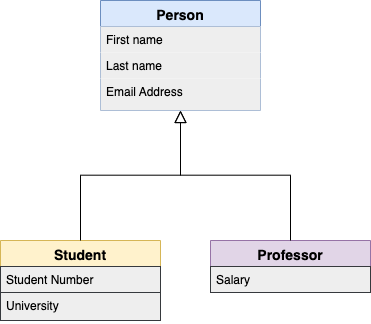
\includegraphics[width=0.5\textwidth]{img/heritage.png}
  \end{center}
\end{frame}

\begin{frame}[fragile]{Exemple : un étudiant est une personne}
\begin{lstlisting}[language=python, numbers=none]
class Person():
    def __init__(self, firstname, lastname):
        self.firstname = firstname
        self.lastname = lastname

    def __str__(self):
        return f"{self.firstname} {self.lastname}"

class Student():
    def __init__(self, firstname, lastname, university):
        self.firstname = firstname
        self.lastname = lastname
        self.university = university        

    def __str__(self):
        return f"{self.firstname} {self.lastname}"
    
    def get_university(self):
        return self.university
\end{lstlisting}
\end{frame}

\begin{frame}[fragile]{Exemple : un étudiant est une personne}
\begin{lstlisting}[language=python, numbers=none]
class Person():
    def __init__(self, firstname, lastname):
        self.firstname = firstname
        self.lastname = lastname

    def __str__(self):
        return f"{self.firstname} {self.lastname}"

class Student():
    def __init__(self, firstname, lastname, university):


        self.university = university        
    



    def get_university(self):
        return self.university
\end{lstlisting}
  \end{frame}


\begin{frame}[fragile]{Définition}

  \begin{itemize}
    \item L'héritage est un mécanisme qui nous permet de créer une nouvelle classe à partir d'une classe existante, en ajoutant de \textcolor{blue}{nouveaux attributs et méthodes}
    \item La nouvelle classe est appelée \textcolor{red}{classe fille} et la classe existante, \textcolor{red}{classe mère}
    \item On dit que la classe fille ``hérite de'' ou  ``étend'' la classe mère
  \end{itemize}

\begin{lstlisting}[language=python, numbers=none]
class mere:
  # corps de la classe mere

class fille(mere):
  # corps de la classe fille
\end{lstlisting}

\end{frame}

\begin{frame}[fragile]{Fonction \texttt{super}}
\begin{lstlisting}[language=python, numbers=none]
class Person():
    def __init__(self, firstname, lastname):
        self.firstname = firstname
        self.lastname = lastname

    def __str__(self):
        return f"{self.firstname} {self.lastname}"

class Student():
    def __init__(self, firstname, lastname, university):


        self.university = university        
    



    def get_university(self):
        return self.university
\end{lstlisting}
  \end{frame}



\begin{frame}[fragile]{Fonction \texttt{super}}
\begin{lstlisting}[numbers=none, morekeywords={Person, super}]
class Person():
    def __init__(self, firstname, lastname):
        self.firstname = firstname
        self.lastname = lastname

    def __str__(self):
        return f"{self.firstname} {self.lastname}"

class Student(Person):
    def __init__(self, firstname, lastname, university):
        super().__init__(firstname, lastname)

        self.university = university        
    



    def get_university(self):
        return self.university
\end{lstlisting}
  \end{frame}

\begin{frame}[fragile]{Fonction \texttt{super}}
\begin{lstlisting}[numbers=none, morekeywords={Person, super}]
class Person():
    def __init__(self, firstname, lastname):
        self.firstname = firstname
        self.lastname = lastname

    def __str__(self):
        return f"{self.firstname} {self.lastname}"

class Student(Person):
    def __init__(self, firstname, lastname, university):
        Person.__init__(self, firstname, lastname)

        self.university = university        
    



    def get_university(self):
        return self.university
\end{lstlisting}
  \end{frame}


\section{Ce qu'il faut retenir}

\begin{frame}{Ce qu'il faut retenir de la programmation objet 1/2}

  \begin{itemize}
    \item C'est un concept central en python : \textcolor{red}{tout est objet}
    \item Elle est équivalente à définir des \textcolor{red}{types}
    \item C'est un manière de \textcolor{red}{stocker de l'information}
    \item Les attributs et les méthodes sont systématiquement \textcolor{red}{publiques}
    \item Il est possible de \textcolor{red}{surcharger} des opérateurs mathématiques (somme, produit, opérateurs logiques, etc.) pour des types non standards
    \item L'héritage permet de partager des attributs et des méthodes entre plusieurs objets et éviter la \textcolor{red}{duplication de code}
  \end{itemize}
\end{frame}



\begin{frame}{Ce qu'il faut retenir de la programmation objet 2/2}

  Exemples pratiques en ML :
  
  \bigskip
  
  \textbf{Data loader en traitement de l'image}

    \href{https://keras.io/examples/vision/oxford_pets_image_segmentation/}{keras.io/examples/vision/oxford\_pets\_image\_segmentation}

  \bigskip

  \textbf{Définition d'un réseau de neurones avec \texttt{PyTorch}}
    
  \href{https://pytorch.org/tutorials/beginner/basics/buildmodel_tutorial.html}{pytorch.org/tutorials/beginner/basics/buildmodel\_tutorial.html}

  \end{frame}


\begin{frame}{Pour aller plus loin}

  \textbf{Concept de polymorphisme}
  
  \href{https://www.w3schools.com/python/python\_polymorphism.asp}{w3schools.com/python/python\_polymorphism}
  
  \medskip

  \textbf{Classes abstraites}
  
  \href{https://peps.python.org/pep-3119/}{peps.python.org/pep-3119}

  \medskip  

  \textbf{Classes de données}
  
  \href{https://docs.python.org/3/library/dataclasses.html}{docs.python.org/3/library/dataclasses}
\end{frame}


\end{document}